<h1 id="sec:weight-decay">Chapter 3: Training transformers with enforced Lipschitz constants</h1>


So far the focus of the metrized deep learning method has been toward the controlling the gradients. Yet if all we control are the gradients, the weights may drift, and the model may become highly sensitive to input and weight perturbations. This sensitivity has been linked to pathologies such as vulnerability to adversarial examples, divergent training, and overfitting. Therefore, this chapter applies the metrized deep learning method to enforce norm constraints on the weights, specifically for transformers, where the closest related work, LipsFormer, only enforces constraints at initialization [<a href="https://arxiv.org/abs/2304.09856" target="_blank" rel="noopener noreferrer" class="citation">Qi et al., 2023</a>]. To explore this gap, we propose and benchmark novel, computationally-efficient tools for maintaining norm-constrained weight matrices. Applying these tools, we are able to train transformer models with Lipschitz bounds enforced throughout training. We find that optimizer dynamics matter: switching from AdamW to Muon improves standard methods---weight decay and spectral normalization---allowing models to reach equal performance with a lower Lipschitz bound. Inspired by Muon's update having a fixed spectral norm, we co-design a weight constraint method that improves the Lipschitz vs. performance tradeoff on MLPs and 2M parameter transformers. Our 4-Lipschitz transformer on Shakespeare text reaches validation accuracy 60\%. Scaling to 145M parameters, our 600-Lipschitz transformer reaches 21\% accuracy on internet text. However, to match the NanoGPT baseline validation accuracy of 39.4\%, our Lipschitz upper bound increases to $10^{274}$. Nonetheless, our Lipschitz transformers train without stability measures such as layer norm, QK norm, and logit tanh softcapping.

\vspace{1em}

\textit{Contribution statement: This chapter adapts material from an upcoming paper. Jeremy Bernstein had the idea to study Lipschitz neural networks from the metrized deep learning perspective. I proposed using odd polynomial iterations to control the singular values of the weights, designed the spectral soft cap method depicted in <a class="cref" data-target="fig:odd-poly-family" href="#fig:odd-poly-family">fig:odd-poly-family</a>, and derived the formula to couple its decay to the learning rate. I contributed to all the experiments in this chapter. I designed the experiment pipeline and ran thousands of CIFAR-10 runs, thousands of Shakespeare transformer runs, and around fifty 145M parameter runs at the NanoGPT scale. Several collaborators joined near the end of the project: Andrii Zahorodnii investigated adversarial robustness (<a class="cref" data-target="fig:accuracy_vs_epsilon" href="#fig:accuracy_vs_epsilon">fig:accuracy_vs_epsilon</a>); Preston Hess invented the spectral hammer method with Andrew Hutchison, compared methods (<a class="cref" data-target="fig:fullmuoncomp" href="#fig:fullmuoncomp">fig:fullmuoncomp</a>), and wrote up several sections of the paper; Franz Cecista contributed innumerable speedrun experiments and fixed an error in the Lipschitz constant calculation; Jeremy Bernstein and Phillip Isola advised throughout.}


<h2 id="subsec:lipschitz-enforced-introduction"> 3.1: Introduction</h2>

Lipschitz constants for neural networks---intuitively, bounds on the sensitivity of each component and of the overall model to input perturbations---are of interest for their effect on generalization and robustness [<a href="https://arxiv.org/abs/1706.08498" target="_blank" rel="noopener noreferrer" class="citation">Bartlett et al., 2017</a>; <a href="https://arxiv.org/abs/1802.04034" target="_blank" rel="noopener noreferrer" class="citation">Tsuzuku et al., 2018</a>] and for applications such as differential privacy [<a href="https://arxiv.org/abs/2305.16202" target="_blank" rel="noopener noreferrer" class="citation">B{\'e}thune et al., 2024</a>]. Seminal work [<a href="https://arxiv.org/abs/1511.06464" target="_blank" rel="noopener noreferrer" class="citation">Arjovsky et al., 2016</a>; <a href="https://arxiv.org/abs/1704.08847" target="_blank" rel="noopener noreferrer" class="citation">Cisse et al., 2017</a>; <a href="https://arxiv.org/abs/1705.10941" target="_blank" rel="noopener noreferrer" class="citation">Yoshida & Miyato, 2017</a>; <a href="https://arxiv.org/abs/1811.05381" target="_blank" rel="noopener noreferrer" class="citation">Anil et al., 2019b</a>] enforces Lipschitz constants beyond initialization for MLPs, RNNs, and GANs, but for transformers, the closest related work, LipsFormer [<a href="https://arxiv.org/abs/2304.09856" target="_blank" rel="noopener noreferrer" class="citation">Qi et al., 2023</a>], does not constrain weights while training. Without constraints, large-scale transformer training may encounter instabilities, which has been attributed to attention and output logits growing too large [<a href="https://arxiv.org/abs/2309.14322" target="_blank" rel="noopener noreferrer" class="citation">Wortsman et al., 2023</a>; <a href="arXiv:2302.05442" target="_blank" rel="noopener noreferrer" class="citation">Dehghani et al., 2023</a>]. Can enforced Lipschitz constants benefit transformers, too? Specifically, we ask:

\begin{center}
    \textit{Can transformers with small, enforced Lipschitz bounds perform well?\\
    How does the weight constraint method affect the Lipschitz vs. performance tradeoff?}
\end{center}

Enforcing Lipschitz bounds on a transformer is challenging because transformers include components that are not globally Lipschitz, such as self-attention [<a href="https://arxiv.org/abs/2006.04710" target="_blank" rel="noopener noreferrer" class="citation">Kim et al., 2021</a>]. We build on <a href="https://arxiv.org/abs/2411.04330" target="_blank" rel="noopener noreferrer" class="citation">Large et al. (2024</a>) who, similar to LipsFormer, enable Lipschitz continuity by reparameterizing residual connections and modifying self-attention; however, the full story is elusive. LipsFormer goes further than <a href="https://arxiv.org/abs/2411.04330" target="_blank" rel="noopener noreferrer" class="citation">Large et al. (2024</a>) to eliminate layer norm [<a href="https://arxiv.org/abs/1607.06450" target="_blank" rel="noopener noreferrer" class="citation">Ba et al., 2016</a>], but the \href{https://github.com/IDEA-Research/LipsFormer/blob/main/models/lipsformer_swin.py#L205-L206}{official implementation} may make Lipschitz bounds impossible by setting $\epsilon = 0$ in QK norm [<a href="https://arxiv.org/abs/2010.04245" target="_blank" rel="noopener noreferrer" class="citation">Henry et al., 2020</a>]. In contrast, we remove activation normalization to explore whether training can proceed with no stability measures.

To develop a toolkit for training transformers with an enforced Lipschitz constant, in <a class="cref" data-target="sec:comparing-methods" href="#sec:comparing-methods">Section 3.2</a> we compare several methods for constraining weight norm. Surprisingly, we find that optimizer choice matters: standard methods such as weight decay [<a href="https://proceedings.neurips.cc/paper/1991/file/8eefcfdf5990e441f0fb6f3fad709e21-Paper.pdf" target="_blank" rel="noopener noreferrer" class="citation">Krogh & Hertz, 1991</a>] and spectral normalization [<a href="https://arxiv.org/abs/1705.10941" target="_blank" rel="noopener noreferrer" class="citation">Yoshida & Miyato, 2017</a>] improve a Lipschitz vs. performance tradeoff more with Muon [<a href="https://kellerjordan.github.io/posts/muon/" target="_blank" rel="noopener noreferrer" class="citation">Jordan et al., 2024</a>] than with AdamW [<a href="https://arxiv.org/abs/1711.05101" target="_blank" rel="noopener noreferrer" class="citation">Loshchilov & Hutter, 2019</a>]. We see improvement under Muon for MLPs trained on CIFAR-10 [<a href="http://www.cs.toronto.edu/~kriz/cifar.html" target="_blank" rel="noopener noreferrer" class="citation">Krizhevsky et al., 2009</a>] and corroborate it on 2M parameter transformers trained on Shakespeare text [<a href="https://github.com/karpathy/nanoGPT" target="_blank" rel="noopener noreferrer" class="citation">Karpathy, 2022</a>].

Beyond standard methods, we are inspired by a property of Muon---its weight updates have small, known spectral norm---to design a weight constraint method called \textit{spectral soft cap}, which enforces a desired maximum spectral norm $\sigma_\text{max}$ by approximating the map $\sigma \mapsto \min(\sigma_\text{max}, \sigma)$ on all singular values $\sigma$ in parallel by iterating odd polynomials on the weights. <a class="cref" data-target="thm:spectral-soft-cap-bound" href="#thm:spectral-soft-cap-bound">thm:spectral-soft-cap-bound</a> proves that spectrally capping the singular values bounds weight norm when training with Muon; we provide no theoretical guarantee for AdamW because the spectral norm of its update is not controlled. For AdamW, we explore a second technique that may be better suited to low stable rank updates, although we do not provide provable guarantees. At every step, this technique finds the largest weight singular value and sets it to $\sigma_\text{max}$. In analogy with a hammer that strikes the nail that sticks out the most, we call this technique \textit{spectral hammer}. Our experiments suggest that the most effective combination is Muon with spectral normalization or spectral soft cap, while from Adam the only technique that elicits a competitive performance vs. Lipschitz tradeoff is spectral hammer.

In <a class="cref" data-target="sec:enforcing-for-transformers" href="#sec:enforcing-for-transformers">Section 3.3</a>, we scale up enforced weight constraint methods to the NanoGPT speedrun benchmark [<a href="https://github.com/KellerJordan/modded-nanogpt" target="_blank" rel="noopener noreferrer" class="citation">Jordan et al., 2024</a>], training 145M parameter transformers to competitive performance without layer norm or QK norm. We train a $600$-Lipschitz transformer to 21.2\% validation accuracy, compared to the non-Lipschitz baseline of 39.4\% validation accuracy. However, to reach a competitive accuracy of 38.2\%, our global Lipschitz upper bound becomes astronomical at $10^{127}$. While <a href="https://arxiv.org/abs/1906.04893" target="_blank" rel="noopener noreferrer" class="citation">Fazlyab et al. (2019</a>) describe ways to tighten Lipschitz bounds, inspecting the maximum activation norms reveals that our model operates far from the worst case. On a particular batch of 393K tokens, the non-Lipschitz baseline has maximum activation entry 148,480 while the $10^{127}$-Lipschitz transformer has maximum activation entry 96.5. Empirically small activations in Lipschitz-constrained transformers may present an opportunity for low-precision training and inference.

\vspace{1em}

\textbf{Our contributions are as follows:}
\begin{itemize}
    \item We train transformers with enforced Lipschitz constraints up to 145M parameters, including a 600-Lipschitz transformer with 21\% accuracy on FineWeb10B internet text and a 4-Lipschitz transformer with 60\% accuracy on Shakespeare text.
    \item We present evidence that weight decay and spectral normalization yield greater benefits when trained with Muon compared to AdamW, matching accuracy with lower Lipschitz bound. We verify standard robustness properties hold when training with Muon.
    \item We introduce two weight norm constraint techniques: \textit{spectral soft cap} and \textit{spectral hammer}. Out of weight regularization methods for AdamW, spectral hammer elicits the most competitive Lipschitz-constrained performance. For Muon, we prove spectral soft cap bounds weight norm and find that it performs similarly or slightly better than spectral normalization. 
\end{itemize}


<h2 id="sec:comparing-methods"> 3.2: Weight norm constraints to enforce a Lipschitz constant</h2>

A function $f(x)$ has Lipschitz constant $K$ under a norm $\norm{\cdot}$ if it satisfies $\norm{f(x_1) - f(x_2)} \leq K \cdot \norm{x_1 - x_2}$ for all inputs $x_1, x_2$. For neural networks, the most common operation is matrix multiplication which has $\ell_2$ Lipschitz constant equal to the spectral norm of the weight matrix. Constraining the spectral norm of weight matrices is not new, with past work primarily exploring weight decay, spectral normalization, and orthogonal constraints [<a href="https://proceedings.neurips.cc/paper/1991/file/8eefcfdf5990e441f0fb6f3fad709e21-Paper.pdf" target="_blank" rel="noopener noreferrer" class="citation">Krogh & Hertz, 1991</a>; <a href="https://arxiv.org/abs/1705.10941" target="_blank" rel="noopener noreferrer" class="citation">Yoshida & Miyato, 2017</a>; <a href="https://arxiv.org/abs/1802.05957" target="_blank" rel="noopener noreferrer" class="citation">Miyato et al., 2018</a>; <a href="https://arxiv.org/abs/1804.04368" target="_blank" rel="noopener noreferrer" class="citation">Gouk et al., 2020</a>; <a href="https://kexue.fm/archives/10648" target="_blank" rel="noopener noreferrer" class="citation">Su, 2024</a>]. These methods have been tested with the AdamW optimizer and have shown benefits for generalization and adversarial robustness [<a href="https://arxiv.org/abs/1706.08498" target="_blank" rel="noopener noreferrer" class="citation">Bartlett et al., 2017</a>; <a href="https://arxiv.org/abs/1802.04034" target="_blank" rel="noopener noreferrer" class="citation">Tsuzuku et al., 2018</a>]. The Muon optimizer introduces new possibilites by ensuring small, fixed-norm weight updates. Inspired by this property, we revisit existing methods and develop new methods for constraining weights. We ask the question:

\begin{center}
    \textit{What is the best way to enforce weight norm constraints throughout training?}
\end{center}

We compare seven methods based on how well they 1) maintain high performance, 2) enforce weight norm constraints, and 3) trade off performance with a Lipschitz bound. To summarize our conclusions, we find that the Muon optimizer achieves lower Lipschitz constants and better performance compared to AdamW. Among the constraint methods, our experiments suggest that spectral soft cap, spectral hard cap, and spectral normalization meet these criteria best.

\textbf{Muon enables hard weight constraints.} Unlike in AdamW, the weight update norm in Muon is bounded by the learning rate---if its orthogonalizing polynomial never exceeds 1. We follow [<a href="https://x.com/YouJiacheng/status/1893704552689303901" target="_blank" rel="noopener noreferrer" class="citation">You, 2025</a>] to ensure this property in our experiments. <a href="https://arxiv.org/abs/2502.07529" target="_blank" rel="noopener noreferrer" class="citation">Pethick et al. (2025</a>) noted that bounded weight update spectral norm upgrades weight decay with parameter $\lambda$ to enforce a \textit{strict} spectral norm constraint of $1/\lambda$. The reason is that an equilibrium occurs between the update step and weight decay when the weight norm $w$ satisfies $w = w(1 - \lambda \eta) + \eta$ for learning rate $\eta > 0$. See <a class="cref" data-target="app:spectral-softcap" href="#app:spectral-softcap">Section 3.5.1</a> for details. We hypothesize that this property may explain our evidence that Muon, compared to AdamW, improves the Lipschitz vs. performance tradeoff for standard methods such as weight decay.

\textbf{A spectral generalization of weight decay.} Weight decay can be viewed as a special case of an \textit{odd polynomial iteration} applied to the weights. Odd polynomials are special because they act directly on the singular values: $p(U \Sigma V^\top) = U p(\Sigma) V^\top$, where $U\Sigma V^\top$ is a singular value decomposition. The odd polynomial for weight decay is $p(x) = (1 - \eta \lambda) x$, where $\eta$ is the learning rate and $\lambda$ is the weight decay. <a href="https://arxiv.org/abs/1704.08847" target="_blank" rel="noopener noreferrer" class="citation">Cisse et al. (2017</a>) explored an orthogonalizing polynomial $p(x) = (1 + \beta)x - \beta x^3$, but <a href="https://arxiv.org/abs/1802.05957" target="_blank" rel="noopener noreferrer" class="citation">Miyato et al. (2018</a>) note that pressuring all singular values toward one limits information in the spectrum. Their method, \textit{spectral normalization}, enforces norm constraints while allowing singular values less than 1 [<a href="https://arxiv.org/abs/1804.04368" target="_blank" rel="noopener noreferrer" class="citation">Gouk et al., 2020</a>], but normalization accomplishes the constraint by scaling down the entire spectrum. This global effect motivates a more targeted approach
: penalizing only the singular values that are too large, leaving smaller ones untouched. For a desired maximum norm $\sigma_\text{max} \geq 0$, an idealized penalty would apply $\min(\sigma_\text{max}, \sigma)$ to the singular values, but exactly computing the SVD is slow. Odd polynomial iterations serve as a fast and effective approximation. We contribute a family of such approximations called \textit{spectral soft cap} that contains weight decay as a special case. The derivation and discussion is in <a class="cref" data-target="app:spectral-softcap" href="#app:spectral-softcap">Section 3.5.1</a>.

<h3 id="sec:methods_weight_constraints">Section 3.2.1: Methods for controlling weight norm</h3>

We are interested in controlling the $\rms \to \rms$ operator norm---a rescaled spectral norm---which has emerged as natural for deep learning [<a href="https://arxiv.org/abs/2310.17813" target="_blank" rel="noopener noreferrer" class="citation">Yang et al., 2023</a>; <a href="https://arxiv.org/abs/2410.21265" target="_blank" rel="noopener noreferrer" class="citation">Bernstein & Newhouse, 2024b</a>]. Unit $\rms\to\rms$ norm is equivalent to a spectral norm of $\sqrt{d_\mathsf{out}/d_\mathsf{in}}$ for a weight matrix $W \in \R^{d_\mathsf{out} \times d_\mathsf{in}}$. In what follows, we denote the principal singular vector subspace with singular value $\sigma_1 \geq 0$ by $\sigma_1 u_1 v_1^\top$, computed via power iteration. We briefly review some known methods to constrain weight norm, then introduce two new methods called spectral capping and spectral hammer.

\textbf{Weight decay}, or Frobenius norm regularization, maps $W \mapsto (1 - \lambda \eta)W$ where $\lambda > 0$ is the decay parameter and $\eta > 0$ is the learning rate, guaranteeing a norm bound in conjunction with Muon.

\textbf{Spectral weight decay}, or spectral norm regularization, targets only the top singular value, mapping $W \mapsto W - \lambda \sigma_1 u_1 v_1^\top$ where $\lambda > 0$ is the decay parameter [<a href="https://arxiv.org/abs/1705.10941" target="_blank" rel="noopener noreferrer" class="citation">Yoshida & Miyato, 2017</a>; <a href="https://kexue.fm/archives/10648" target="_blank" rel="noopener noreferrer" class="citation">Su, 2024</a>].

\textbf{Spectral normalization}, originally introduced in GAN training [<a href="https://arxiv.org/abs/1802.05957" target="_blank" rel="noopener noreferrer" class="citation">Miyato et al., 2018</a>], guarantees a spectral norm bound by mapping $W \mapsto \tfrac{W}{\sigma_1}$.

\textbf{Stiefel manifold projection} pressures all singular values toward 1 using an odd polynomial iteration $W \mapsto p(W)$, leaving open the choice of polynomial $p$. We follow <a href="https://x.com/YouJiacheng/status/1893704552689303901" target="_blank" rel="noopener noreferrer" class="citation">You (2025</a>) whose polynomial converges very rapidly rather than the polynomial from [<a href="https://arxiv.org/abs/1704.08847" target="_blank" rel="noopener noreferrer" class="citation">Cisse et al., 2017</a>]. Although Stiefel manifold projections usually refers to projections for rectangular matrices, with a slight abuse of notation we use it to describe this operation on both square and rectangular matrices.

\vspace{1em}

We extend these ideas with two new methods:

\vspace{1em}

\textbf{Spectral hammer} is similar to spectral weight decay, but sets the top singular value to $\sigma_\text{max}$ by mapping $W \mapsto W + (\sigma_\text{max} - \sigma_1)u_1v_1^\top$---so to speak, a hammer that strikes the nail that sticks out the most [<a href="https://deep-learning-mit.github.io/staging/blog/2023/WeightDecaySpecNormEffects/" target="_blank" rel="noopener noreferrer" class="citation">Hess & Hutchison, 2023</a>]. Spectral hammer does not guarantee the spectral norm stays below $\sigma_\text{max} > 0$ because multiple singular vectors may increase per update. Spectral hammer is better suited to low stable rank weight updates as are common in Adam [<a href="https://arxiv.org/abs/2403.14958" target="_blank" rel="noopener noreferrer" class="citation">Zhao et al., 2024</a>]. Muon's update is always high stable rank.

\textbf{Spectral capping} is co-designed for Muon's high stable rank update, smoothly approximating the map $\sigma \mapsto \min(\sigma_\text{max}, \sigma)$ for all singular values in parallel. Rather than rely on costly SVDs, it uses an odd polynomial approximation. The primary variant we experiment with is called \textit{spectral soft cap} because it applies a loose approximation $p_2(p_1(x))$, where $p_1(x) = x - \alpha x^3$ and $p_2(x) = x + \alpha x^3$ with strength parameter $\alpha \geq 0$, as depicted in <a class="cref" data-target="fig:odd-poly-family" href="#fig:odd-poly-family">fig:odd-poly-family</a> in <a class="cref" data-target="subsec:a-primitive-for-controlling-singular-values" href="#subsec:a-primitive-for-controlling-singular-values">Section 1.2</a>. To incorporate weight decay as a special case, we may first apply $p_0(x) = (1 - \lambda \eta) x$. This composition is designed to decay a singular value very little when $\sigma \ll \sigma_\text{max}$, but when $\sigma = \sigma_\text{max}$ to decay it as strongly as necessary to counteract Muon's known update norm, strictly enforcing a weight norm bound. When the learning rate is scheduled, finding the minimal $\alpha \geq 0$ that bounds the weight norm avoids accumulating error.

\begin{theorembox}[Spectral soft cap bounds spectral norm.]
    \label{thm:spectral-soft-cap-bound}
    Given a desired maximum spectral norm $\sigma_\text{max} \geq 0$, learning rate $\eta \geq 0$, weight decay $\lambda \geq 0$, and weight matrix with bounded norm $\norm{W}_\ast \leq \sigma_\text{max}$, there is a minimal $\alpha \geq 0$ such that Muon's update step followed by spectral soft cap preserves $\norm{W}_\ast \leq \sigma_\text{max}$. Calculating $\alpha$ involves solving the roots of a quartic polynomial.
\end{theorembox}

<a class="cref" data-target="app:spectral-softcap" href="#app:spectral-softcap">Section 3.5.1</a> gives the proof. A second variant of spectral capping is \textit{spectral hard cap}, which uses four quintic polynomials that closely approximate $\min(\sigma_\text{max}, \sigma)$, as depicted in <a class="cref" data-target="fig:spectral-hard-cap-graph" href="#fig:spectral-hard-cap-graph">fig:spectral-hard-cap-graph</a> in <a class="cref" data-target="app:spectral-softcap" href="#app:spectral-softcap">Section 3.5.1</a>. Because this approximation is fixed, errors can compound later in training when the learning rate is scheduled to $0$.

Together, these methods cover a range of tradeoffs between strict norm enforcement, preserving the spectrum, and computational efficiency. There may be other, better approaches, and we think exploring alternatives is an exciting direction. Note that spectral soft cap and spectral hard cap are designed to be compatible with Muon and therefore were not applied to tests with AdamW.

\begin{figure}[t]
  \centering
  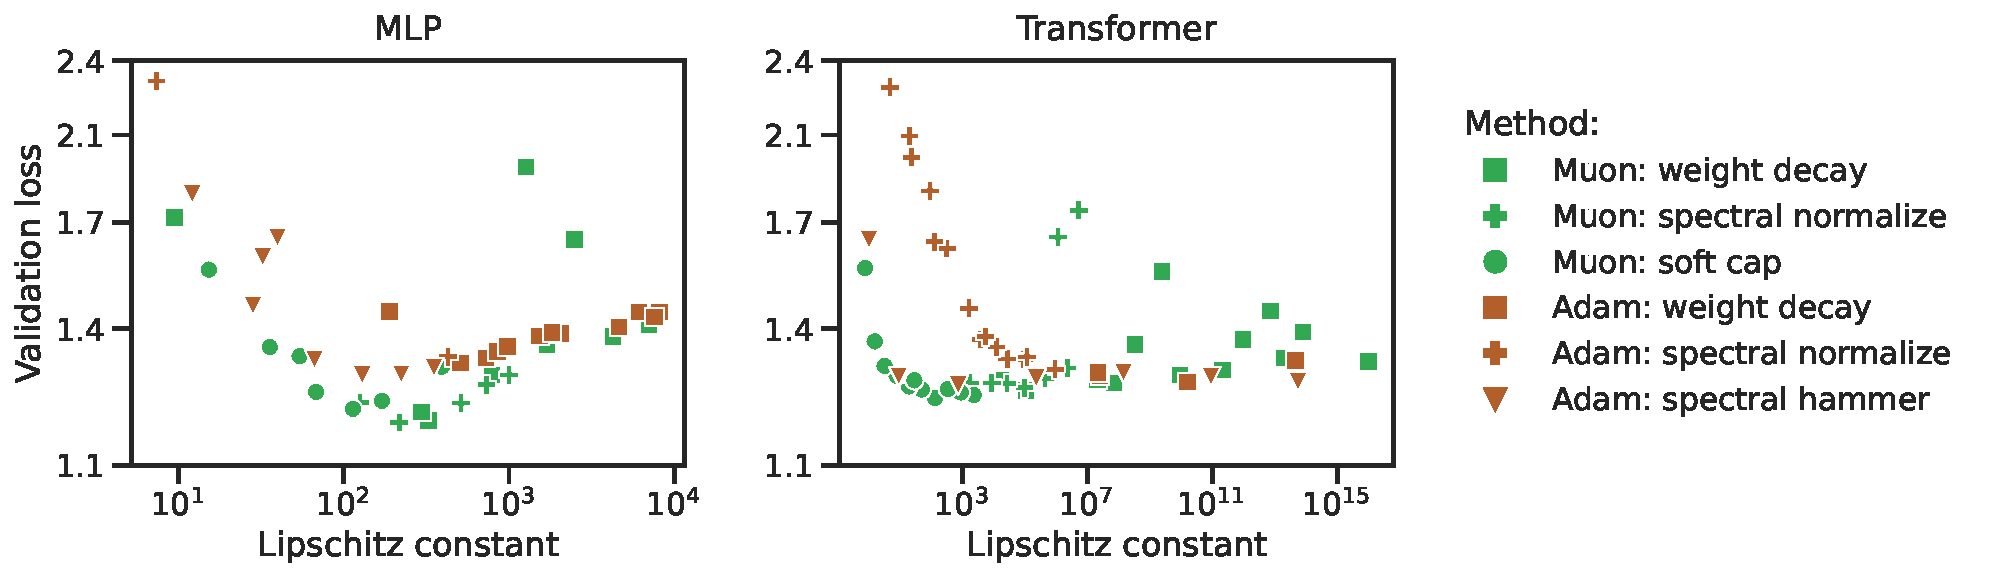
\includegraphics[width=\linewidth]{figure/weight-decay/pareto_val_loss_vs_lipschitz_combined.pdf}
  \caption{\textbf{Using Muon instead of AdamW improves the Lipschitz vs. performance tradeoff for standard weight regularization techniques.} We train 1600 MLPs on CIFAR-10 (left) and 800 transformers on Shakespeare text (right), varying the optimizer and weight constraint method. Weight decay and spectral normalization reach better loss with lower Lipschitz constant when using Muon. Two weight constraint methods that we design---spectral soft cap and spectral hammer---are also promising. See <a class="cref" data-target="app:experimental-details" href="#app:experimental-details">Section 3.5.3</a> for experimental details.}
  \label{fig:pareto}
\end{figure}

\subsection{AdamW and Muon: comparing weight constraint methods}

In <a class="cref" data-target="fig:pareto" href="#fig:pareto">fig:pareto</a>, we run a sweep to map the tradeoff frontier between validation loss and Lipschitz constant across our methods. The Lipschitz constants are calculated with respect to the $\rms\to\rms$ operator norm (<a class="cref" data-target="sec:methods_weight_constraints" href="#sec:methods_weight_constraints">Section 3.2.1</a>). For a $\mathsf{ReLU}$ MLP, the Lipschitz constant is the product of the $\rms\to\rms$ norms of its weights. For a transformer, the Lipschitz constant is calculated as described in <a class="cref" data-target="subsec:lipschitz-constant-of-transformer" href="#subsec:lipschitz-constant-of-transformer">Section 3.3.2</a>. Muon consistently achieves both lower validation loss \textit{and} lower Lipschitz constants than AdamW, a trend that holds for MLPs on CIFAR-10 and transformers on Shakespeare text. This result motivates our choice to adopt Muon for larger-scale experiments. Spectral normalization and spectral soft cap appear to make the most efficient use of a Lipschitz budget. Spectral hammer--which is designed for AdamW's low stable rank weight updates--shows competitive performance but does not enforce a Lipschitz constant, limiting its reliability for settings where constraint enforcement is critical. The sweep includes 2400 training runs, where for each method we display only the best validation loss per bin of Lipschitz constant.

\subsection{Adversarial robustness of Lipschitz networks}

Prior work [<a href="https://arxiv.org/abs/1704.08847" target="_blank" rel="noopener noreferrer" class="citation">Cisse et al., 2017</a>; <a href="https://arxiv.org/abs/2111.01395" target="_blank" rel="noopener noreferrer" class="citation">Huang et al., 2021</a>] suggests that a neural network's adversarial robustness is related to its Lipschitz constant, making Lipschitz control a potential path for developing models with high certified accuracy. We confirm this relationship holds for MLPs trained with Muon and spectral soft cap. <a class="cref" data-target="fig:accuracy_vs_epsilon" href="#fig:accuracy_vs_epsilon">fig:accuracy_vs_epsilon</a> compares the accuracy of two trained MLPs under various budgets of adversarial perturbation $\epsilon$. The pair depicted has matching accuracy $\approx$ 45\% but different Lipschitz constants: $15.2$ (Muon + spectral soft cap) vs. $7618.8$ (AdamW + weight decay).

While both models achieve similar accuracy without perturbation, the Lipschitz-constrained MLP (quantified in the RMS $\rightarrow$ RMS operator norm, <a class="cref" data-target="sec:methods_weight_constraints" href="#sec:methods_weight_constraints">Section 3.2.1</a>) trained with Muon exhibits a smoother dropoff in accuracy and confidence across the $2000$ CIFAR-10 test set images as the adversarial attack increases its $l_2$ perturbation. Larger values of $\epsilon$ are required to fool the Lipschitz-constrained network (Figure \ref{fig:accuracy_vs_epsilon}, left).

\begin{figure}[t]
    \centering
    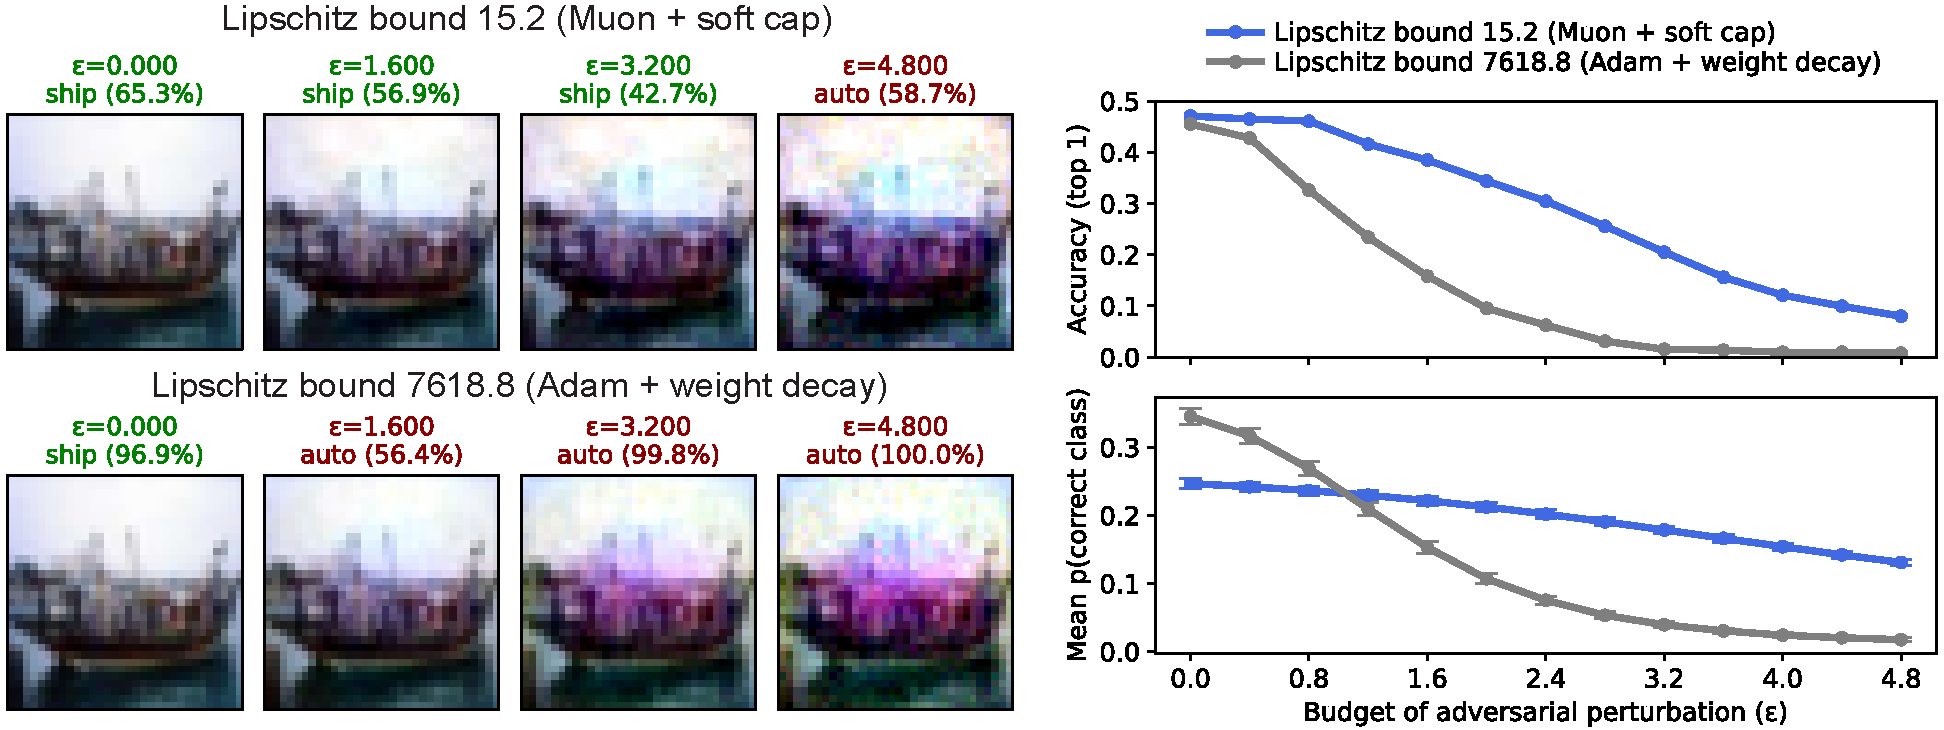
\includegraphics[width=1.0\linewidth]{figure/weight-decay/accuracy_epsilon_cifar.pdf}
    \caption{\textbf{Networks trained with Muon and spectral soft cap have lower Lipschitz bounds and are more adversarially robust.} 
    Lower Lipschitz constants have been linked to greater adversarial robustness %\jeremy{could there not be counter-examples to this? could we weaken the claim} 
    [<a href="https://arxiv.org/abs/1704.08847" target="_blank" rel="noopener noreferrer" class="citation">Cisse et al., 2017</a>; <a href="https://arxiv.org/abs/2111.01395" target="_blank" rel="noopener noreferrer" class="citation">Huang et al., 2021</a>]. To assess this effect in our models, we train a CIFAR-10 MLP with a Lipschitz constant of 15.2 (Muon + spectral soft cap), which matches the 45\% clean accuracy of a baseline model (AdamW + weight decay) that has a a higher Lipschitz constant of 7618.8. 
    Left: Example adversarial attacks with different $\ell_2$ budget $\epsilon \geq 0$ for the perturbation. 
    Top right: We quantify adversarial robustness across 2000 test images by the top-1 accuracy as a function of $\epsilon$. 
    The Lipschitz-constrained network trained with Muon and spectral soft cap maintains a higher accuracy for larger values of $\epsilon$. 
    Bottom right: the mean probability of the correct class in the Lipschitz-constrained network starts lower than that of the baseline model, but degrades slowly under increasing $\epsilon$. By contrast, the baseline model peaks higher for $\epsilon=0$, but drops off sharply.
    }
    \label{fig:accuracy_vs_epsilon}
\end{figure}

\subsection{Comparing weight constraint methods within Muon} 

In <a class="cref" data-target="fig:fullmuoncomp" href="#fig:fullmuoncomp">fig:fullmuoncomp</a>, we use Muon alongside all seven weight constraint methods to identify which approaches best meet three goals: 1) enabling us to define a Lipschitz constant before training, 2) enforcing that constant throughout training, and 3) matching or exceeding the performance of standard weight decay. We tested each weight constraint method on a 3-layer MLP with hidden dimension 256, trained with Muon on CIFAR-10 classification. Full experimental details are in <a class="cref" data-target="app:experimental-details" href="#app:experimental-details">Section 3.5.3</a>.

In <a class="cref" data-target="fig:fullmuoncomp" href="#fig:fullmuoncomp">fig:fullmuoncomp</a> (left panel), we see that spectral normalization, spectral soft cap, and spectral hard cap define the frontier of the Lipschitz vs. validation loss tradeoff. In <a class="cref" data-target="fig:fullmuoncomp" href="#fig:fullmuoncomp">fig:fullmuoncomp</a> (middle), we select the parameter settings with the highest validation accuracy for further analysis. Spectral normalization, spectral soft cap, and spectral hard cap are the only methods to reach within 1\% validation accuracy of the baseline (Muon with weight decay). Other methods reached within 4\% accuracy.

<a class="cref" data-target="fig:fullmuoncomp" href="#fig:fullmuoncomp">fig:fullmuoncomp</a> (right panel) visualizes how the norm of the hidden weight matrix evolves during training. All methods but spectral hammer retain the weight norm at or under its target. In contrast, spectral hammer exceeds its target but begins to converge near the end, indicating that it could be a promising technique under Muon, too, on longer training runs that also schedule learning rate to 0. However, within our 50-epoch window, it fails to reliably control the Lipschitz constant. Spectral weight decay does not enforce predefined Lipschitz constants, so it is not plotted.

We select spectral soft cap, spectral hard cap, and spectral normalization for our transformer training experiments. While all weight constraint methods could potentially benefit from combining with standard weight decay, we want to isolate the effect of each one.

\begin{figure}[t]
    \centering
    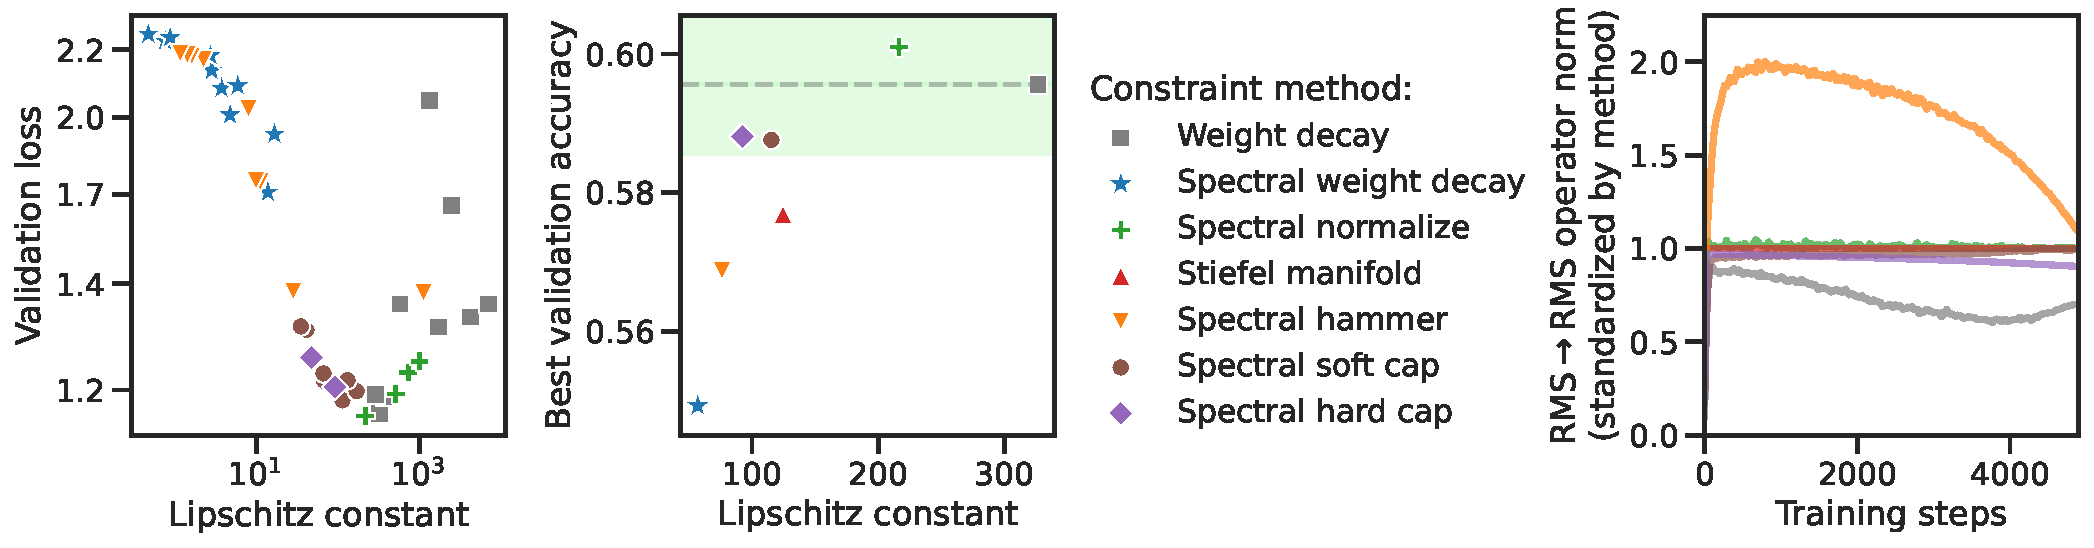
\includegraphics[width=1.0\linewidth]{figure/weight-decay/full_moun_comparision.pdf}
    \caption{\textbf{Left: Weight constraint methods designed for Muon lie on the frontier of the Lipschitz vs. loss tradeoff.} Each point shows the lowest validation loss achieved at a given Lipschitz constant across all MLP runs on CIFAR-10. In the low loss regime, staying on the tradeoff frontier requires either spectral normalization or spectrally capping the singular values. \textbf{Middle: Spectral normalization and spectral capping match baseline with lower Lipschitz constant on CIFAR-10.} Each method comes within 1\% accuracy (shaded green region) and has lower Lipschitz constant. \textbf{Right: RMS $\boldsymbol{\to}$ RMS operator norm of hidden layers over training for the best networks.} The norm is standardized so that the weight constraints all target 1. Spectral normalization and Stiefel manifold projection strictly meet this target. Weight decay, spectral soft cap, and spectral hard cap stay below the target, while spectral hammer fails to remain constrained.}
    \label{fig:fullmuoncomp}
\end{figure}


<h2 id="sec:enforcing-for-transformers"> 3.3: Transformers with enforced weight constraints</h2>

To develop a toolkit for training Lipschitz-constrained transformers, we begin in <a class="cref" data-target="subsec:architecture" href="#subsec:architecture">Section 3.3.1</a> with a discussion of how to handle residual connections and self-attention. In <a class="cref" data-target="subsec:lipschitz-constant-of-transformer" href="#subsec:lipschitz-constant-of-transformer">Section 3.3.2</a>, we explain how to calculate a Lipschitz bound for a transformer. In <a class="cref" data-target="subsec:shakespeare" href="#subsec:shakespeare">Section 3.3.3</a>, we find that spectral normalization and spectral soft cap perform well on 2M parameter transformers trained on Shakespeare text. In <a class="cref" data-target="subsec:nanogpt" href="#subsec:nanogpt">Section 3.3.4</a>, we scale up to a transformer with 145M parameters trained on FineWeb10B internet text [<a href="https://arxiv.org/abs/2406.17557" target="_blank" rel="noopener noreferrer" class="citation">Penedo et al., 2024</a>]. To combat the undertuned baseline problem, we begin from the competitive benchmark of NanoGPT speedrunning [<a href="https://github.com/KellerJordan/modded-nanogpt" target="_blank" rel="noopener noreferrer" class="citation">Jordan et al., 2024</a>].

<h3 id="subsec:architecture">Section 3.3.1: Breaking the multiplication barrier?</h3>

A major triumph of <a href="https://arxiv.org/abs/2411.04330" target="_blank" rel="noopener noreferrer" class="citation">Large et al. (2024</a>) is to create transformers with a depth-independent Lipschitz constant. However, their approach relies on activations having unit $\rms$ norm. Because we will later relax this constraint, our transformers will typically \textit{not} have a depth-independent Lipschitz bound. Nonetheless, we use their two architectural suggestions.

\textbf{Reparameterizing residual connections.} The classic residual connection from <a href="https://arxiv.org/abs/1512.03385" target="_blank" rel="noopener noreferrer" class="citation">He et al. (2015</a>) defines the update $x + \mathsf{block}(x)$, but even a 1-Lipschitz block can exponentially increase the Lipschitz constant: $x + \mathsf{identity}(x)$ doubles at every layer. <a href="https://arxiv.org/abs/2411.04330" target="_blank" rel="noopener noreferrer" class="citation">Large et al. (2024</a>) use a convex combination <div id="" class="equation">    \label{eq:breaking-barrier-convex-combination}
    \frac{N-1}{N} \cdot x + \frac{1}{N} \cdot\mathsf{block}(x)</div>to break this multiplication barrier,  where $N$ is the number of layers. The residual connection will be $1$-Lipschitz if the block is $1$-Lipschitz. See Proposition 4 of <a href="https://arxiv.org/abs/2411.04330" target="_blank" rel="noopener noreferrer" class="citation">Large et al. (2024</a>). Our experiments use this convex parameterization. However, the bound breaks down if activation norms exceed 1. We are unable to attain high performance without relaxing the 1-Lipschitz constraint. Therefore we do not fully break the multiplication barrier: deeper networks can accrue astronomical Lipschitz bounds.

\textbf{Attention with $\boldsymbol{1/d}$ scaling.} The original multihead attention of <a href="https://arxiv.org/abs/1706.03762" target="_blank" rel="noopener noreferrer" class="citation">Vaswani et al. (2017</a>) has no global Lipschitz bound [<a href="https://arxiv.org/abs/2006.04710" target="_blank" rel="noopener noreferrer" class="citation">Kim et al., 2021</a>]. In a footnote, <a href="https://arxiv.org/abs/1706.03762" target="_blank" rel="noopener noreferrer" class="citation">Vaswani et al. (2017</a>) indicate that they chose $1/\sqrt{d}$ scaling because two random vectors $u, v$ with mean $0$ and variance $1$ will have a dot product $u \cdot v$ with mean $0$ and variance the dimension $d$. But key and query vectors may align more than at random. Perfect alignment would suggest $1/d$ scaling. <a href="https://arxiv.org/abs/2411.04330" target="_blank" rel="noopener noreferrer" class="citation">Large et al. (2024</a>) prove that $1/d$ scaling in the softmax, together with a factor of $\tfrac13$, makes functional attention, <div id="" class="equation">    \label{eq:breaking-barrier-softmax-1-d}
    \frac13 \times \text{softmax}\left(\frac{QK^\top}{d}\right)V,</div> 1-Lipschitz if the input norms are 1. The Lipschitz constant is with respect to the $\norm{\cdot}_{\rms\infty}$ norm, the max $\rms$ norm of any token. See Proposition 7 of <a href="https://arxiv.org/abs/2411.04330" target="_blank" rel="noopener noreferrer" class="citation">Large et al. (2024</a>). Finally, while <a href="https://arxiv.org/abs/2411.04330" target="_blank" rel="noopener noreferrer" class="citation">Large et al. (2024</a>) retains layer normalization, we remove it so that every operation is Lipschitz continuous.

<h3 id="subsec:lipschitz-constant-of-transformer">Section 3.3.2: Calculating the Lipschitz constant of a transformer</h3>

To test whether transformers with small Lipschitz constant can perform well, we would like to know what weight norm to enforce to end up with a desired Lipschitz bound. This section sketches an algorithm for bounding the Lipschitz constant of a transformer given its weight norms; the full algorithm is in <a class="cref" data-target="app:lipschitz-attention" href="#app:lipschitz-attention">Section 3.5.2</a>. Our bound tightens Theorem 2 from LipsFormer [<a href="https://arxiv.org/abs/2304.09856" target="_blank" rel="noopener noreferrer" class="citation">Qi et al., 2023</a>] by accounting for each weight norm individually, rather than working with the max weight norm across residual blocks. <a href="https://arxiv.org/abs/1906.04893" target="_blank" rel="noopener noreferrer" class="citation">Fazlyab et al. (2019</a>) suggest ways to tighten a global bound like ours, which we leave to future work. To bound self-attention, we extend Proposition 7 from the modular norm paper [<a href="https://arxiv.org/abs/2411.04330" target="_blank" rel="noopener noreferrer" class="citation">Large et al., 2024</a>] to when the input is no longer unit norm, an essential concession to reach different regions of the Lipschitz vs. performance tradeoff.

Our Lipschitz bounds are with respect to the max $\rms$ norm over token positions, denoted $\norm{\cdot}_{\infty\rms}$.

\textbf{Step 1: Bound activation norms.} Our Lipschitz bound for rescaled dot-product attention relies on the activation norms remaining bounded. Therefore, the algorithm begins by computing a per-layer bound for the maximum $\norm{\cdot}_{\infty\rms}$ norm of activations. This bound comes from combining residual connections with per-block maximum activation increases, found for an MLP by multiplying its two weight norms and for attention by multiplying its $W_V$ and $W_O$ weight norms. Our MLPs can slightly decay activation norm because we scale $\mathsf{GeLU}$ down by its maximum derivative, $\mathsf{GeLU}/1.1289$.

\textbf{Step 2: Bound the Lipschitz constant.} Suppose the Lipschitz constant prior to reaching a particular layer is $L$. The Lipschitz constant after a residual connection is at most $(1 - \alpha) L + \alpha \cdot L \cdot L_\mathsf{block}$. To compute a block's Lipschitz constant $L_\mathsf{block}$, for MLPs we calculate $\norm{W_\mathsf{in}}_{\rms\to\rms} \cdot \norm{W_\mathsf{out}}_{\rms\to\rms} / 1.1289$ due our rescaled $\mathsf{GeLU}$, and for attention we use the formula from <a class="cref" data-target="thm:function-attention-is-lipschitz" href="#thm:function-attention-is-lipschitz">thm:function-attention-is-lipschitz</a>.

<h3 id="subsec:shakespeare">Section 3.3.3: Shakespeare Transformer</h3>

Before scaling to NanoGPT, we explore the Lipschitz vs. performance tradeoff for transformers at a smaller scale. To narrow our aim, we want a transformer that has small Lipschitz constant \textit{at every layer}. <a href="https://arxiv.org/abs/2104.05097" target="_blank" rel="noopener noreferrer" class="citation">B{\'e}thune et al. (2022</a>) comments that any $L$-Lipschitz classifier can be made $1$-Lipschitz by dividing the logits by $L$, but we do not downscale our final logits, although scaling temperature during training could have beneficial effects [<a href="https://arxiv.org/abs/2010.07344" target="_blank" rel="noopener noreferrer" class="citation">Agarwala et al., 2023</a>]. All experimental details are available in <a class="cref" data-target="app:experimental-details" href="#app:experimental-details">Section 3.5.3</a>.

\textbf{We can train a competitive 4-Lipschitz Shakespeare transformer.} Our 4-Lipschitz transformer reaches validation loss $1.29 < 1.47$ from the baseline in <a href="https://github.com/karpathy/nanoGPT" target="_blank" rel="noopener noreferrer" class="citation">Karpathy (2022</a>), although the baseline may not be tuned carefully. Our model has dimension 256, depth 3, and was trained for 2000 steps with Muon; the baseline has dimension 384, depth 6, and was trained for 5000 steps with AdamW. Ours uses no layer normalization. To achieve this performance requires relaxing the maximum weight norm $\sigma_\text{max}$ to around 2. The best validation loss from our sweep was 1.20 with a 131-Lipschitz transformer. While gains may be attributed to hyperparameters or optimizer choice, we nonetheless end up with one construction of our aim: a performant transformer with a small, enforced Lipschitz bound.

<h3 id="subsec:nanogpt">Section 3.3.4: Scaling to NanoGPT</h3>

We validate our method by training a transformer with 145M parameters on the NanoGPT speedrun benchmark [<a href="https://github.com/KellerJordan/modded-nanogpt" target="_blank" rel="noopener noreferrer" class="citation">Jordan et al., 2024</a>], which is built on top of [<a href="https://github.com/karpathy/nanoGPT" target="_blank" rel="noopener noreferrer" class="citation">Karpathy, 2022</a>]'s reproduction of GPT-2. The baseline is competitively optimized to reach validation loss 3.28 in the shortest wallclock time. The latest record as of February 1, 2025 requires only 1770 training steps, or 3 minutes of training on an 8xH100, and achieves a validation accuracy of 39.4\%. We implement our methods on top of this baseline while keeping all other training methods fixed. We report the validation loss and the validation accuracy as primary comparison metrics.

To implement our method, we first remove speedrun-specific optimizations such as skip connections and learnable scale parameters. Next we remove the layer norms used for pre-normalization, the logit tanh softcap, and the QK norms in the attention layers. We also replace the $\mathsf{ReLU}^2$ activations with $\mathsf{GeLU}/1.1289$---making the activation function Lipschitz continuous. We reparametrize the residual connections and attention layer as in <a class="cref" data-target="eq:breaking-barrier-convex-combination,eq:breaking-barrier-softmax-1-d" href="#eq:breaking-barrier-convex-combination,eq:breaking-barrier-softmax-1-d">eq:breaking-barrier-convex-combination,eq:breaking-barrier-softmax-1-d</a>. At initialization, we project the linear weights to be semi-orthogonal and normalize the embeddings to have $\rms$ norm 1. Finally, we explicitly extend beyond the closest related work, LipsFormer [<a href="https://arxiv.org/abs/2304.09856" target="_blank" rel="noopener noreferrer" class="citation">Qi et al., 2023</a>], by enforcing weight norm constraints throughout training: we cap the $\rms$ norm of embeddings to 1 and apply one of the weight constraint methods from <a class="cref" data-target="sec:methods_weight_constraints" href="#sec:methods_weight_constraints">Section 3.2.1</a> to all other weights after every training step.

\begin{table}[tbp]
    \centering
    \resizebox{\textwidth}{!}{
    \renewcommand{\arraystretch}{1.1}
    \begin{tabular}{lcrcccc}
        \toprule
        \makecell[l]{\textbf{Transformer}\\\textbf{Architecture}} &
        \makecell[c]{\textbf{Lipschitz}\\\textbf{Bound}} &
        \makecell[r]{\textbf{Number}\\\textbf{of Steps}} &
        \makecell[c]{\textbf{Weight}\\\textbf{Constraint}} &
        \makecell[c]{\textbf{Validation}\\\textbf{Accuracy} ($\uparrow$)} &
        \makecell[c]{\textbf{Validation}\\\textbf{Loss} ($\downarrow$)} &
        \makecell[c]{\textbf{Activation}\\\textbf{Max Entry}} \\ % \textbf{Max Activation RMS}
        \midrule
        Baseline (speedrun) & $\infty$ & 1{,}770 & none & \textbf{0.394} & \textbf{3.280} & 148{,}480 \\ % 12{,}480.0 &
        Baseline (Karpathy) & $\infty$ & 17{,}000 & none & - & \textbf{3.280} & - \\
        \midrule
        LipsFormer & $10^{130}$ & 1{,}770 & none & 0.301 & 4.130 & 61.1 \\ % ? & 11.31
        Ours ($\sigma_\text{max}=1$) & $600$ & 1{,}770 & spectral normalize & 0.212 & 5.047 & 14 \\
        Ours ($\sigma_\text{max}=8$) & $10^{118}$ & 1{,}770 & spectral soft cap & \textbf{0.365} & \textbf{3.569} & 54.25 \\
        Ours ($\sigma_\text{max}=8$) & $10^{56}$ & 1{,}770 & spectral hard cap & 0.354 & 3.670 & 107 \\
        Ours ($\sigma_\text{max}=8$) & $10^{130}$ & 1{,}770 & spectral normalize & 0.360 & 3.607 & 100 \\
        \midrule
        Ours ($\sigma_\text{max}=16$) & $10^{274}$ & 7{,}080 & spectral normalize & \textbf{0.395} & \textbf{3.280} & 160 \\
        \bottomrule
    \end{tabular}
    }
    \vspace{0.6em}
    \caption{\textbf{Transformers with enforced Lipschitz constraints can match performance on NanoGPT.} The NanoGPT speedrun is a competitively tuned benchmark building on Karpathy's original replication of GPT-2 [<a href="https://github.com/karpathy/nanoGPT" target="_blank" rel="noopener noreferrer" class="citation">Karpathy, 2022</a>; <a href="https://github.com/KellerJordan/modded-nanogpt" target="_blank" rel="noopener noreferrer" class="citation">Jordan et al., 2024</a>]. With the speedrun baseline as a starting point, we substitute Lipschitz transformer components and constrain weight norms to not exceed a given $\sigma_\text{max} \geq 0$. Unlike LipsFormer [<a href="https://arxiv.org/abs/2304.09856" target="_blank" rel="noopener noreferrer" class="citation">Qi et al., 2023</a>], our weight constraint methods enforce a Lipschitz constant chosen prior to training. To demonstrate, we train a 600-Lipschitz transformer to $21.2\%$ accuracy. However, reaching accuracy on par with the baseline increases the Lipschitz bound to $10^{274}$, computed as in <a class="cref" data-target="subsec:lipschitz-constant-of-transformer" href="#subsec:lipschitz-constant-of-transformer">Section 3.3.2</a>. Our Lipschitz bounds may be loose, as suggested by the small maximum activation that we observe across a batch of 393K tokens. Per-run loss variance is 0.0008.}
    \label{tab:nanogptspeedrun}
\end{table}

<a class="cref" data-target="tab:nanogptspeedrun" href="#tab:nanogptspeedrun">tab:nanogptspeedrun</a> summarizes our 145M parameter scale transformer results. In contrast to LipsFormer, our method guarantees a Lipschitz upper bound specified prior to training. An important lever is the maximum $\rms\to\rms$ norm $\sigma_\text{max} \geq 0$ we allow for the linear layers. Smaller $\sigma_\text{max}$ correspond to smaller Lipschitz bounds but may lower performance, and vice versa. Two other variables that affect the Lipschitz constant are the attention logit scale and final logit scale. Using spectral normalization with $\sigma_\text{max}=1$ and a final logit scale of 8 results in a 600-Lipschitz transformer that attains validation loss 5.047 and accuracy 21.2\%. No activation in this model exceeds $\rms$ norm 1, which could enhance stability during training. Setting $\sigma_\text{max}=16$ enables reaching parity with the speedrun performance but increases the Lipschitz bound to $10^{276}$. This setting trains for $4\times$ as many steps as the current speedrun record (but $2.4\times$ fewer than Karpathy's baseline).


<h2 id="sec:discussion"> 3.4: Discussion</h2>

Despite high Lipschitz upper bounds, our transformers on NanoGPT exhibit low maximum activation entries (50-110) compared to the baseline (148K). Perhaps as a result, our models train stably without standard measures including layer norm, QK norm, or tanh logit softcapping. In future work, we are interested to test whether these low maximum activations hold potential for low-precision training and inference. We also wonder whether training would remain stable at larger scales.

For MLPs and small transformers, we find that using Muon improves the Lipschitz vs. performance tradeoff. Out of weight constraint methods we test, \textit{spectral normalization}, \textit{spectral soft cap}, and \textit{spectral hard cap} compare favorably to standard weight decay. Perhaps surprisingly, on both CIFAR-10 and Shakespeare data, we achieve our best loss with Lipschitz-enforced models, potentially representing a training speed benefit.

Our work has several limitations. We did not find a principled way to select weight norm, final logit scale, and attention logit scale hyperparameters, instead relying on sweeps. Our Lipschitz bound also increases rapidly as depth increases, unless we constrain weights to unit norm. A different architecture, or insight beyond a global Lipschitz bound, could make progress on this problem.

In conclusion, this paper develops a method for training transformers with an enforced Lipschitz constant throughout training, extending earlier efforts focused on different architectures or only constraints at initialization. Lipschitz-certified transformers may be of interest for domains such as privacy, control, adversarial robustness, and low-precision training. Although training speed benefits fade in our NanoGPT speedrun experiments, we wonder whether at this scale Lipschitz-enforced training can be made faster than standard training.


<h2 id="subsec:catch-all-appendix"> 3.5: Proofs and experimental details</h2>


<h3 id="app:spectral-softcap">Section 3.5.1: Coupling spectral cap to learning rate</h3>

This section proves <a class="cref" data-target="thm:spectral-soft-cap-bound" href="#thm:spectral-soft-cap-bound">thm:spectral-soft-cap-bound</a>: spectral soft cap bounds weight norm. We will derive a strength parameter that couples to the learning rate, because otherwise using odd polynomial approximation---rather than the ideal map $\min(\sigma_\text{max}, \sigma)$---accumulates errors when the learning rate falls below the approximation gap. We will prove the theorem using an equilbrium analysis: solving for the fixed point of a contractive map.

To warm up, there is a special case in which weight decay provably bounds the weight norm during training. It happens when the norm of the update is bounded by the learning rate, $\norm{\Delta W} \leq \eta$. To see why, suppose weight decay is applied at every step of training and is linearly coupled to the learning rate as $\lambda \eta$ for some constant $\lambda > 0$. Subadditivity of norms guarantees $\norm{W + \Delta W} \leq \norm{W} + \norm{\Delta W} \leq \norm{W} + \eta$. The weights cannot increase further when the decay and the learning rate are in equilbrium: $\norm{W} \cdot (1 - \lambda \eta) + \eta = \norm{W}$. The equilibrium occurs at $\norm{W} = 1/\lambda$. Therefore $1/\lambda$ is the maximum weight norm possible under standard weight decay, if the update norm is bounded above by $\eta$. <a href="https://arxiv.org/abs/2502.07529" target="_blank" rel="noopener noreferrer" class="citation">Pethick et al. (2025</a>) noted the same phenomenon.

To prove <a class="cref" data-target="thm:spectral-soft-cap-bound" href="#thm:spectral-soft-cap-bound">thm:spectral-soft-cap-bound</a>, we conduct a general equilibrium analysis to consider three effects: weight decay, optimizer step, and weight projection. The net effect of the three effects should decrease every singular value $\sigma \geq \sigma_\text{max}$. Let the weight decay $\lambda$ be coupled to the learning rate $\eta$. Suppose the weight update is constrained to have norm $\norm{\Delta W} \leq \eta$. Let $p(x)$ be an odd polynomial. Equilbrium occurs when <div id="" class="equation">    \label{eq:equilibrium}
    p(x \cdot (1 - \lambda \eta) + \eta) \leq x.</div> In words, apply weight decay, apply an optimizer step that will not increase singular values by more than $\eta$, and then apply the odd polynomial. If the singular value does not increase for all $x \in [0, \sigma_\text{max}]$, then the weight norm will never exceed $\sigma_\text{max}$.

Recall that $p_1(x) = x - \alpha x^3$ and $p_2(x) = x + \alpha x^3$.

When $p(x) = p_2(p_1(x))$, the equilibrium condition <a class="cref" data-target="eq:equilibrium" href="#eq:equilibrium">eq:equilibrium</a> becomes \begin{gather}
    f(\alpha) = \left(k-\alpha k^{3}\right)+\alpha\left(k-\alpha k^{3}\right)^{3} - \sigma_\text{max} \leq 0, \\
    \text{where } \; k = \sigma_\text{max} \cdot (1 - \lambda \eta) + \eta.
\end{gather} We can consider only $x = \sigma_\text{max}$ because, in this case, larger $x$ will decrease if a smaller $x$ decreases. Here $\alpha$ is the free variable. Finding the smallest $\alpha > 0$ amounts to solving the quartic polynomial <div id="" class="equation">    \label{eq:generalized-coupling}
    -k^9 \alpha^4 + 3k^7 \alpha^3 - 3k^5 \alpha^2 + k - \sigma_\text{max} = 0.</div> Any numerical solver can approximate $\alpha$. This is the $\alpha$ that makes $\sigma_\text{max}$ a fixed point under the overall training step. Connecting to the earlier equilibrium analysis, the special case $\alpha = 0$ is possible when already $k = \sigma_\text{max}$, or $\sigma_\text{max} = 1/\lambda$. While the coupling for spectral soft capping is not linear as in common implementations of AdamW, it succeeds at making tight weight norm bounds compatible with learning rate schedules that may tend to $0$. Initializing the weights near $\sigma_\text{max}$, rather than strictly less than it, suffices for the bound to hold throughout training in practice.

One limitation of automatic coupling is that it may be stronger than necessary, because it assumes updates align perfectly with the weights in the worst case. If the learning rate is scheduled to $0$, gradients may align less with the existing weights especially at the end, which can cause the weight norm to contract slightly.

\begin{figure}[t]
    \centering
    \subfloat{
        \includesvg[width=0.4\textwidth]{figure/newton-schulz/franz-hard-cap-components.svg}
    }
    \hspace{0.03\textwidth}
    \subfloat{
        \includesvg[width=0.4\textwidth]{figure/newton-schulz/franz-hard-cap.svg}
    }
    \caption{\textbf{Spectral hard cap} is a weight constraint method that applies the above odd polynomial to a weight matrix, which applies it to all singular values in parallel. Left: the four quintic polynomials. Right: the composition of the four quintic polynomials is designed to approximate $\min(1, x)$ on the range $x \in [0, 3]$.}
    \label{fig:spectral-hard-cap-graph}
\end{figure}



<h3 id="app:lipschitz-attention">Section 3.5.2: Proving an upper bound on the Lipschitz constant of a transformer</h3>

We elaborate on the algorithm sketched in <a class="cref" data-target="subsec:lipschitz-constant-of-transformer" href="#subsec:lipschitz-constant-of-transformer">Section 3.3.2</a> and prove a Lipschitz bound on attention. Our Lipschitz bounds are with respect to the max $\rms$ norm over token positions, denoted $\norm{\cdot}_{\infty\rms}$.

Recall the two primary ways Lipschitz constants $L_f$ and $L_g$ of two functions $f$ and $g$ interact:
\begin{itemize}
    \item \textbf{Adding:} $f + g$ has Lipschitz constant at most $L_f + L_g$.
    \item \textbf{Composing:} $f \circ g$ has Lipschitz constant at most $L_f \cdot L_g$.
\end{itemize}

\textbf{Step 1: Residual connections.} Suppose that, before reaching a certain residual connection, a transformer maps input data $x$ to $f(x)$ with Lipschitz constant $L$. Suppose the transformer has $2N$ residual connections. Let $\alpha = \tfrac{1}{2N}$. The residual connection acts on $f(x)$ as <div id="" class="equation">    \left[ (1 - \alpha) \cdot \mathsf{identity} + \alpha \cdot \mathsf{block} \right](f(x)).</div> After the residual connection, the Lipschitz constant composes and adds to become at most <div id="" class="equation">    (1 - \alpha) \cdot L + \alpha \cdot L \cdot L_\mathsf{block}.</div> Applying this formula sequentially upper bounds the Lipschitz constant of a transformer layer by layer. We now determine $L_\mathsf{block}$ for an MLP and attention block in terms of their weight norms.

\textbf{Step 2: MLP.} Our MLP composes $W_\mathsf{out} \circ (\mathsf{GeLU} / 1.1289) \circ W_\mathsf{in}$. The Lipschitz constants of the two weight matrices are their norms $\norm{W_\mathsf{out}}_{\rms\to\rms}$ and $\norm{W_\mathsf{in}}_{\rms\to\rms}$, while $\mathsf{GeLU} / 1.1289$ has Lipschitz constant $1$ because we divide by the maximum derivative of $\mathsf{GeLU}$. Overall, the Lipschitz bound for an MLP block is $L_\mathsf{MLP} \leq \norm{W_\mathsf{out}}_{\rms\to\rms} \norm{W_\mathsf{in}}_{\rms\to\rms} / 1.1289$.

\textbf{Step 3: Attention.} Let $\ell$ denote the token dimension. Let the queries, keys, and values be denoted by $(q, k, v) \in \R^{\ell \times d_Q} \times \R^{\ell \times d_Q} \times \R^{\ell \times d_V}$. Our attention block composes <div id="" class="equation">    \tfrac13 W_\mathsf{out} \circ F,</div> where function attention is denoted by $F = \softmax(\tfrac{1}{d_Q} qk^\top + M)v$ for some mask $M$. As a consequence of the following theorem, if every attention input is unit norm, then functional attention is $1$-Lipschitz. This property is what motivates scaling attention by $\tfrac{1}{d_Q}$ rather than $\tfrac{1}{\sqrt{d_Q}}$ inside the softmax. It also motivates scaling the attention output by $\tfrac{1}{3}$ to make it unit sensitivity. Functional attention is no longer $1$-Lipschitz if its inputs are not unit norm. Recall that the shorthand notation $\norm{x}_{\infty\rms}$ is the max RMS norm of a $d$-dimensional activation over $l$ tokens, $x \in \R^{\ell \times d}$.

\begin{theorembox}[Lipschitz bound on functional attention]
    \label{thm:function-attention-is-lipschitz}
    Let $\diamond$ denote tensor contraction. Given any perturbations $\Delta q, \Delta k, \Delta v$ to the queries, keys, and values, functional attention satisfies <div id="" class="equation">    \norm{\nabla F(q, k, v) \diamond (\Delta q, \Delta k, \Delta v)} \leq \norm{\Delta v} + \norm{v} (\norm{\Delta q} \norm{k} + \norm{q} \norm{\Delta k}),</div> where the norm is $\norm{\cdot}_{\infty \rms} : \R^{\ell \times d} \to \R$, the max-over-tokens $\rms$ norm of the embedding vector.
\end{theorembox}

\begin{proof}
    The argument mirrors the proof of Proposition 7 from the modular norm paper [<a href="https://arxiv.org/abs/2411.04330" target="_blank" rel="noopener noreferrer" class="citation">Large et al., 2024</a>]. We write the attention matrix as $A = \softmax(\tfrac{1}{d_Q} qk^\top + M)$. Its derivative is $\Delta A = \nabla_{(q,k)} \softmax(\tfrac{1}{d_Q} qk^\top + M) \diamond (\Delta q, \Delta k)$. The derivative of $F$ splits into two terms, \begin{equation}
        \label{eq:attention-lipschitz}
        \nabla F(q, k, v) \diamond (\Delta q, \Delta k, \Delta v) = A (\Delta v) + (\Delta A) v.
    \end{equation} We call the maximum entry of $A$ or $\Delta A$ its $L^\infty$ operator norm, which comes into play by observing that $\norm{Ax}_{\infty\rms} \leq \norm{A}_{\infty-\mathsf{op}} \norm{x}_{\infty\rms}$. For the first term, note that $\norm{A}_{\infty-\mathsf{op}} \leq 1$ because softmax never exceeds $1$. For the second term, <a href="https://arxiv.org/abs/2411.04330" target="_blank" rel="noopener noreferrer" class="citation">Large et al. (2024</a>) in Equation E.58 show that \begin{equation}
        \norm{\Delta A}_{\infty-\mathsf{op}} \leq \norm{\Delta q}_{\infty\rms} \norm{k}_{\infty\rms} + \norm{q}_{\infty\rms} \norm{\Delta k}_{\infty\rms}.
    \end{equation} The result follows by applying these bounds to $\norm{A}_{\infty-\mathsf{op}} \norm{\Delta v}_{\infty\rms} + \norm{\Delta A}_{\infty-\mathsf{op}} \norm{v}_{\infty\rms}$.
\end{proof}

\textbf{Step 4. Activation norm bounds.} To apply the theorem, we now bound the input norm to attention. To do so we will track the maximum $\rms$ norm of activations everywhere in the network. We do not use layer norm and therefore cannot reset activation norms to 1. Let $x_0, \dots, x_{2N}$ denote all the activations, from the initial embedding $x_0$ through to the $N$ alternating attention and MLP blocks acting via residual connections. Suppose the embedding layer maps tokens to have $\rms$ norm at most $1$, or $\norm{x_0}_{\infty\rms} \leq 1$. Attention and MLP increase the norm as follows:
\begin{itemize}
    \item Attention computes $W_\mathsf{out} \circ (V, A)$ for some attention matrix $A$, where $(V, A)$ is shorthand for functional attention. By definition $V$ cannot increase the $\rms$ norm of the embedding $x_i$ at any token by more than its $\rms\to\rms$ operator norm, meaning $\norm{V x_i}_{\infty\rms} \leq \norm{V}_{\rms\to\rms} \norm{x_i}_{\infty\rms}$. The same bound applies to $(V, A)x_i$ by subadditivity of norms, since entries of the attention matrix $A$ sum to $1$ in the token dimension. Therefore attention can increase the activation norm by \begin{equation}
        \norm{(W_\mathsf{out} \circ (V, A))x_i}_{\infty\rms} \leq \norm{W_\mathsf{out}}_{\rms\to\rms} \norm{V}_{\rms\to\rms} \norm{x_i}_{\infty\rms}.
    \end{equation} In words, multiply the weight norms of $W_\mathsf{out}$ and $V$ to get the maximum increase.
    \item The MLP computes $W_\mathsf{out} \circ (\mathsf{GeLU} / 1.1289) \circ W_\mathsf{in}$. Therefore the MLP can increase activation norm by $\norm{W_\mathsf{out}}_{\rms\to\rms} \norm{W_\mathsf{in}}_{\rms\to\rms} / 1.1289$, since $|\mathsf{GeLU}(x)| \leq |x|$ for all $x \in \R$.
    \item The residual connection acts like \begin{equation}
        \norm{(1 - \alpha) \cdot x_i + \alpha \cdot \mathsf{block}(x_i)}_{\infty\rms} \leq (1 - \alpha) \norm{x_i}_{\infty \rms} + \alpha \norm{\mathsf{block}(x_i)}_{\infty\rms}.
    \end{equation}
\end{itemize}

\textbf{Algorithm to compute Lipschitz constant.} Therefore, given the weight norms of all matrices in a transformer, we use the preceding results to compute its Lipschitz constant in two steps. First, we upper bound the activation norm everywhere in the network using Step 4. Second, we upper bound the Lipschitz constant using Steps 1-3. The Lipschitz bound after the final layer is what we refer to as the transformer's Lipschitz upper bound.


\subsection{Implementing LipsFormer and bounding its Lipschitz constant}

To turn our enforced norm training into LipsFormer [<a href="https://arxiv.org/abs/2304.09856" target="_blank" rel="noopener noreferrer" class="citation">Qi et al., 2023</a>], we make the following changes:

\begin{enumerate}
    \item Remove spectral soft cap and embed projections.
    \item Use CenterNorm: mean subtraction with learnable entrywise scale and bias.
    \item Use scaled-head cosine attention with $\epsilon = 10^{-6}$, $\tau = 12$, $\nu = 1$. Notably, the \href{https://github.com/IDEA-Research/LipsFormer/blob/main/models/lipsformer_swin.py#L205-L206}{official implementation} of LipsFormer uses $\epsilon = 0$. According to their Theorem 1, this choice may make a finite Lipschitz bound impossible. We set $\epsilon > 0$ to fix the issue.
    \item Heuristically scale down attention output by $1/n_\text{heads}$ to match their implementation.
    \item Insert residual connections with learnable strength $\alpha$, initialized to $1/n_\text{residual\_connections}$.
    \item Xavier normal initialize linear layers, then apply spectral normalization $W \mapsto W / \norm{W}_\ast$.
    \item Include drop path: every residual connection is skipped with $p=0.5$ and, if taken, is scaled up by $1/(1-p)$, matching their official implementation which uses \verb|nn.Dropout|.
    \item Use weight decay 0.1, matching their implementation (not applied to scalar parameters).
    \item Use the Muon optimizer to give LipsFormer the fairest comparison, copying hyperparameters from our run. We tested training with AdamW for all parameters, an exact replication, but found performance degraded sigificantly: after 1770 steps, validation loss was 4.86 (compared to 3.61) and validation accuracy was 0.227 (compared to 0.301).
    \item For non-weight-matrix parameters, use Adam hyperparameters $\eta = 0.001$, $\beta_1 = 0.9$, $\beta_2 = 0.999$, $\epsilon = 10^{-8}$ to match their implementation.
    \item Use cosine learning rate schedule with decay to 0 to match their implementation.
\end{enumerate}

\textbf{Bounding the Lipschitz constant of LipsFormer.} In <a class="cref" data-target="tab:nanogptspeedrun" href="#tab:nanogptspeedrun">tab:nanogptspeedrun</a>, we report that our trained implementation of LipsFormer has a Lipschitz upper bound of $10^{130}$. To calculate this value, we use the final weight norms of the MLP and attention blocks to bound the Lipschitz constant of each residual block, relying on LipsFormer's Theorem 1:
\[
    \mathsf{Lip}(\text{SCSA})_2 \leq 2N(N-1)\nu\tau\epsilon^{-\tfrac12}\norm{W^K}_2 + 2(N-1)\nu\tau\epsilon^{-\tfrac12}\norm{W^Q}_2 + 2N\nu\epsilon^{-\tfrac12}\norm{W^V}_2.
\]
Using $N = 128$ (head dimension), $\tau = 12$, $\nu = 1$, and empirical weight norms, we calculate the Lipschitz constant for every layer. We use the maximum entry of the learned residual strength $\alpha$, which is an entrywise multiplication, to convert the layerwise bounds into a final bound \[
    \mathsf{Lip}(F) \leq \prod_{s=1}^S \prod_{m=1}^S (1 + \alpha_{s,m} \mathsf{Lip}(f_{s,m})),
\] which we take from their Equation 19. Alpha has typical maximum entries around $0.5$ for attention connections and $0.15$ for MLP connections. With $\epsilon = 10^{-6}$, we compute a final Lipschitz bound of $1.97 \times 10^{129}$.


<h3 id="app:experimental-details">Section 3.5.3: Experimental details</h3>

This section gives experimental details for all results in the paper. The three categories of experiments we run are MLP training, Shakespeare transformer training, and NanoGPT speedrun training.

\textbf{Datasets.}
\begin{itemize}
    \item For MLP training we use the CIFAR-10 dataset \cite{krizhevsky2009cifar} with the standard train and test splits and no data augmentation. We do not shuffle the order of batches.
    \item For Shakespeare transformer training we use Karpathy's 1M character-level dataset with standard training and validation splits [<a href="https://github.com/karpathy/nanoGPT" target="_blank" rel="noopener noreferrer" class="citation">Karpathy, 2022</a>]. We shuffle the order of batches.
    \item For NanoGPT speedrun transformer training we use the FineWeb10B dataset [<a href="https://arxiv.org/abs/2406.17557" target="_blank" rel="noopener noreferrer" class="citation">Penedo et al., 2024</a>] loaded in the standard order. We use the same validation split as the modded NanoGPT speedrun benchmark [<a href="https://github.com/KellerJordan/modded-nanogpt" target="_blank" rel="noopener noreferrer" class="citation">Jordan et al., 2024</a>].
\end{itemize}

\textbf{Compute requirement.} All our experiments can run on a V100, A100, or H100 GPU in less than 5 minutes, except the NanoGPT speedrun transformer which requires 8xH100 and runs in 5-10 minutes.

\textbf{Modula library.} For MLP and Shakespeare experiments, we use JAX [<a href="http://github.com/jax-ml/jax" target="_blank" rel="noopener noreferrer" class="citation">Bradbury et al., 2018</a>] on top of the Modula library [<a href="https://arxiv.org/abs/2411.04330" target="_blank" rel="noopener noreferrer" class="citation">Large et al., 2024</a>; <a href="https://docs.modula.systems/" target="_blank" rel="noopener noreferrer" class="citation">Bernstein, 2025</a>]. We implement our own model components. Our AdamW implementation does not include bias correction, although the discrepancy decays rapidly after aronud 20 steps because we use $\beta_1 = 0.9, \beta_2 = 0.95$ in all experiments except one, not reported, in which we determine that this is a good setting for the momentum EMAs.

\textbf{MLP experiments.} All MLPs we train are width 256 and depth 3 (i.e., one hidden layer) with $\mathsf{ReLU}$ activations and no bias on data from CIFAR-10. We use batch size 512 and a linear learning rate schedule that decays to 0 in all experiments. Modula's mass calculation causes the effective learning rate to be scaled by $1/3$. We train for 50 epochs except in one case, when we train for 20 epochs for the models in <a class="cref" data-target="fig:accuracy_vs_epsilon" href="#fig:accuracy_vs_epsilon">fig:accuracy_vs_epsilon</a>. We zero-initialize the final layer. We train all models in float32 precision and run the weight constrain methods in float32 precision. We experimented with lower precision and found comparable metrics across the board for bfloat16 training. We set seed 0 and store all hyperparameters and log information to enhance reproducibility.

\textbf{Shakespeare experiments.} All transformers we train for Shakespeare are width 256 with 3 blocks (attention + MLP), no bias, and four attention heads. The out projection in each attention and MLP block is initialized to zero. We use sequence length 256 and batch size 64 to match the baseline from [<a href="https://github.com/karpathy/nanoGPT" target="_blank" rel="noopener noreferrer" class="citation">Karpathy, 2022</a>], except we train for 2000 steps while Karpathy trains for 5000 steps. We set Modula's blocks mass parameter to 32 to cause 95\% of the feature learning to occur in the transformer blocks. We determined this ratio by sweeping the blocks mass, which controls the ratio of learning rate between the two embedding layers and the transformer blocks. Training with Muon means applying Muon to all linear layer weight matrices (including the final logit head) but normalizing the columns of embedding gradient, as suggested by the $\ell_1 \to \rms$ duality map [<a href="https://arxiv.org/abs/2410.21265" target="_blank" rel="noopener noreferrer" class="citation">Bernstein & Newhouse, 2024b</a>]. We were concerned that rare tokens may cause the momentum buffer to dualize columns to full strength updates for hundreds of steps until the column decays to exactly zero, so we tested whether capping the maximum inflation factor for the embedding column normalization could help. We tested maximum factors in the set $\{1, 4, 16, \dots, 65536\}$ across 8 seeds and found no significant difference. We choose to maximally multiply each column by 16 during the dualization step. Finally, we found that to train to the validation losses reported we had to use a trick: we decayed the learning rate by a factor of 1/2 per residual layer, causing later layers to train more than earlier layers. This change is implemented by setting the sensitivity of the $\mathsf{Mul}$ module in Modula to 1. We do not know why this trick is necessary.

<a class="cref" data-target="fig:pareto" href="#fig:pareto">fig:pareto</a> sweeps over the following hyperparameters:
\begin{itemize}
    \item MLPs on CIFAR-10: we test the following combinations of optimzer and weight constraint method: weight decay, spectral weight decay, spectral hammer, spectral normalization, and Stiefel manifold projection for both AdamW and Muon; and spectral soft cap and spectral hard cap only for Muon. For AdamW, we vary the weight decay and spectral weight decay parameters with 10 points in log-space from $10^{-2}$ to $10^{0}$. For Muon we vary the weight decay parameter with 10 points in log-space from $10^{-3}$ to $10^{0}$ and the spectral weight decay parameter with 10 points in log-space from $10^{-2}$ to $10^{0}$. For AdamW with spectral normalization, Stiefel manifold projection, and spectral hammer, we vary the maximum weight norm in the set $\sigma_\text{max} \in \{2, 3, 4, 5, 6, 7, 8\}$. For Muon with spectral normalization, Stiefel manifold projection, spectral soft cap, and spectral hard cap, we vary the maximum weight norm in the set $\sigma_\text{max} \in \{4, 5, 6, 7, 8, 9, 10\}$. For Muon with spectral hammer we vary the maximum weight norm in the set $\sigma_\text{max} \in \{1, 2, 3, \ldots , 10\}$. For AdamW with all methods we sweep 16 learning rates in log-space between $10^{-5}$ and $10^{-0.5}$. For Muon we sweep 16 learning rates in log-space between $10^{-2}$ and $10^{1}$ for all methods except for spectral hammer, where we use these learning rates for $\sigma_\text{max} \in \{4, 5, 6, 7, 8, 9, 10\}$, and use 16 learning rates in log-space between $10^{-3}$ and $10^{0}$ for  $\sigma_\text{max} \in \{1, 2, 3\}$. Overall, this sweep results in 1,610 total combinations, 682 with AdamW and 928 with Muon.
    \item Transformers on Shakespeare: we test the following combinations of optimizer and weight constraint method: (AdamW, weight decay), (AdamW, spectral normalize), (AdamW, spectral hammer), (Muon, weight decay), (Muon, spectral normalize), (Muon, spectral soft cap). For spectral normalize, spectral hammer, and spectral soft cap, we vary the maximum weight norm in the set $\sigma_\text{max} \in \{1.0, 1.2, \dots, 2.8, 3.0\}$. For the baseline, we vary weight decay in the set $\lambda \in \{2/3, 0.5, 0.4, 0.3, 0.2, 0.1, 0.05, 0.03, 0.01, 0\}$. For AdamW we sweep 16 learning rates between $10^{-4.5}$ and $10^{-1.5}$. For Muon, we sweep 12 learning rates between $10^{-1.5}$ and $10^{1.5}$. We ran tests before to find ranges that cover the optimal learning rate.
\end{itemize}

<a class="cref" data-target="fig:accuracy_vs_epsilon" href="#fig:accuracy_vs_epsilon">fig:accuracy_vs_epsilon</a> reports adversarial examples and dataset-wide statistics from two models trained for 20 epochs. The AdamW model is trained with learning rate $8.1 \times 10^{-3}$ and weight decay $\lambda = 0.1$. The Muon model is trained with learning rate $2.3 \times 10^{-1}$ and weight decay $\lambda = 0$, using the spectral soft cap method with a weight constraint of $\sigma_\text{max} = 3$.

The left panel of <a class="cref" data-target="fig:fullmuoncomp" href="#fig:fullmuoncomp">fig:fullmuoncomp</a> visualizes the same data from the experiment for <a class="cref" data-target="fig:pareto" href="#fig:pareto">fig:pareto</a>, but focuses only on MLPs trained with Muon on CIFAR-10. The middle and right panels use the Muon optimizer, with the following tuples of weight constraint method, maximum singular value, weight decay, spectral weight decay, and learning rate:
\begin{itemize}
    \item Weight decay, N/A, 0.1, 0, 1.585
    \item Spectral weight decay, N/A, 0, 0.05, 0.157
    \item Spectral normalization, 6, 0, 0, 1.0
    \item Stiefel manifold projection, 5, 0, 0, 1.0
    \item Spectral soft cap, 6, 0, 0, 0.398
    \item Spectral hard cap, 5, 0, 0, 0.631
\end{itemize}

\textbf{NanoGPT experiments.} Following the Modded-NanoGPT speedrun standard [<a href="https://github.com/KellerJordan/modded-nanogpt" target="_blank" rel="noopener noreferrer" class="citation">Jordan et al., 2024</a>], our training runs print log files with the full source code required to reproduce the results. We briefly summarize the changes we made to convert the NanoGPT speedrun record (as of May 2025) into our method:
\begin{itemize}
    \item Every step, $\rms$ normalize the embedding columns.
    \item Initialize all linear layer weight matrices to be orthogonal.
    \item Reparameterize residual connections according to <a class="cref" data-target="eq:breaking-barrier-convex-combination" href="#eq:breaking-barrier-convex-combination">eq:breaking-barrier-convex-combination</a>: $\tfrac{L-1}{L} x + \tfrac{1}{L} \mathsf{block}(x)$ residual connections, where $L = 24$ is the number of residual connections.
    \item Reparameterize attention according to <a class="cref" data-target="eq:breaking-barrier-softmax-1-d" href="#eq:breaking-barrier-softmax-1-d">eq:breaking-barrier-softmax-1-d</a>: $\tfrac13$ overall scale on the attention output and $1/d_\text{head}$ scale inside the softmax.
    \item Every step, apply spectral soft cap (or spectral normalize) to every linear layer weight matrix based on a prespecified maximum desired weight norm $\sigma_\text{max}$.
    \item Use different orthogonalization coefficients that at most inflate a singular value to 1.14502. Therefore, the maximum update norm we pass to the strength parameter solver for learning rate coupling in spectral soft cap is $\eta \cdot 1.14502 \cdot 1.05$ with an extra factor of $1.05$ to be safe around numerical precision errors. The iteration is derived by modifying the method in [<a href="http://leloykun.github.io/ponder/muon-opt-coeffs/" target="_blank" rel="noopener noreferrer" class="citation">Cesista et al., 2025</a>].
    \item Remove U-net structure.
    \item Use $\mathsf{GeLU} / 1.1289$ instead of $\mathsf{ReLU}^2$.
    \item Switch dimensional scaling to be $\sqrt{\mathsf{fan\_{out}} / \mathsf{fan\_{in}}}$ instead of $\max(1, \sqrt{\mathsf{fan\_out} / \mathsf{fan\_in}})$.
    \item Remove $\rms$ normalization: the model is now Lipschitz continuous.
    \item Add back the 7th attention layer (which was removed in the speedrun).
    \item Run weight projections in \verb|bfloat16| (which we found to slightly improve performance). Spectral normalization uses 2 iterations, meaning that weight norms can exceed the specified maximum $\sigma_\text{max}$ due to approximation error; in practice weights with norms enforced by spectral normalization exceed the specified maximum by around 10\%.
\end{itemize}